\documentclass{article}
\usepackage[utf8]{inputenc}

\usepackage{amsthm,amssymb,amsmath}
\usepackage{graphicx}
\usepackage{float}

\newcommand{\NN}{\mathbb{N}}
\newcommand{\ZZ}{\mathbb{Z}}
\newcommand{\RR}{\mathbb{R}}
\newcommand{\QQ}{\mathbb{Q}}
\newcommand{\CC}{\mathbb{C}}

\title{AERO7970 - Trajectory Optimiztion \\ {\small Project 01}}
\author{Matt Boler}
\date{\today}

\begin{document}

\maketitle

\begin{abstract}
  This report details the implementation of a fuel-optimal close-proximity rendezvous maneuver.
  The solution was implemented in \texttt{Matlab} using both the built-in \texttt{solve} function and the \texttt{CVX} library.
  Included are performance comparisons and the resulting trajectories and control inputs.
\end{abstract}

%%
\section{Problem Modeling}

We are given the following optimization problem:
\begin{align*}
  \min_{X, U} \quad & \sum_{i=1}^{N-1} ||U_i||_{L1} \\
  \textrm{s.t.} \quad & \dot{X}_t = AX_t + BU_t \\
  & T_{min} \leq U_{i} \leq T_{max} \\
  & X_0 = \begin{bmatrix}
    -1e3 & 0 & 0 & 0 & 0 & 0
  \end{bmatrix} \\
  & X_N = \begin{bmatrix}
    0 & 0 & 0 & 0 & 0 & 0
  \end{bmatrix}
\end{align*}

While the L1-norm is not strictly a linear performance criterion, we can introduce a set of slack variables $S \geq 0$ to bound the control input $U$ and then minimize their sum as an LP problem.
Additionally, we must convert the continuous-time dynamics constraint into a discretized form.
We use a zero-order hold discretization to convert the dynamics:
\begin{align*}
  \dot{X} = AX + BU \rightarrow X_{k+1} = expm(A*dt) X_k + B*dt * U_k
\end{align*}

Restructuring the problem as such results in:
\begin{align*}
  \min_{X, U, S} \quad & \sum_{i = 1}^{N-1} S_i \\
  \textrm{s.t.} \quad & X_{i+1} = expm(A*dt) * X_i + B*dt*U_i \\
  & S_i \geq 0 \\
  & -S_i \leq U_i \leq S_i \\
  & T_{min} \leq U_{i} \leq T_{max} \\
  & X_0 = \begin{bmatrix}
    -1e3 & 0 & 0 & 0 & 0 & 0
  \end{bmatrix} \\
  & X_N = \begin{bmatrix}
    0 & 0 & 0 & 0 & 0 & 0
  \end{bmatrix}
\end{align*}
which was then implemented in problem-based form in \texttt{Matlab} and \texttt{CVX}.

\section{Results}

After implementing the problem in \texttt{Matlab} and \texttt{CVX}, the formulation-to-solution code was timed and averaged over 10 runs.
The average times are shown below in Table \ref{tab:timing}.

\begin{table}[h]
\centering
\begin{tabular}{| l | c |}
  \hline
  Solver & Average Time (s) \\ \hline
  Linprog (Dual-Simplex) & 0.41164 \\
  Linprog (Interior-Point) & 0.22449 \\
  CVX & 0.73741 \\ \hline
\end{tabular}
\caption{Average formulation-to-solution time for considered solvers}
\label{tab:timing}
\end{table}

The resulting trajectories and control inputs are shown below in Figures \ref{fig:trajectories-fuel} and \ref{fig:controls-fuel}.

\begin{figure}[H]
  \centering
  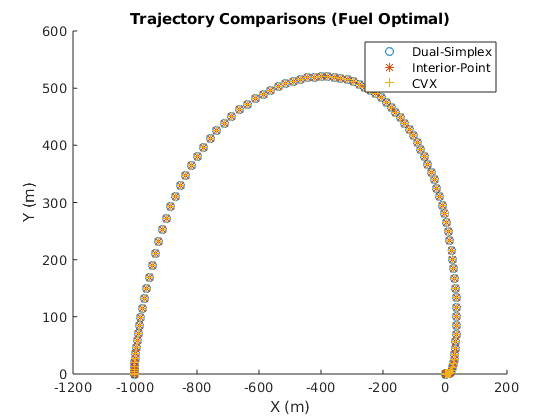
\includegraphics[width=0.7\textwidth]{images/trajectories_fuel.png}
  \caption{Generated fuel-optimal trajectories from each solver}
  \label{fig:trajectories-fuel}
\end{figure}

\begin{figure}[H]
  \centering
  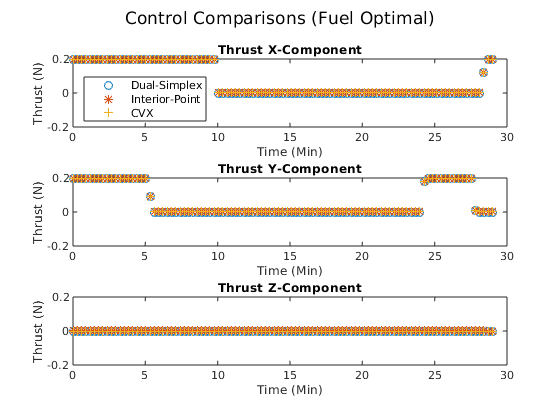
\includegraphics[width=0.7\textwidth]{images/controls_fuel.png}
  \caption{Generated fuel-optimal control inputs from each solver}
  \label{fig:controls-fuel}
\end{figure}

Additionally, it was found that the minimum time needed to perform the maneuver was 21 minutes.
The generated time-optimal trajectories and controls are shown below in Figures \ref{fig:trajectories-time} and \ref{fig:controls-time}.

\begin{figure}[H]
  \centering
  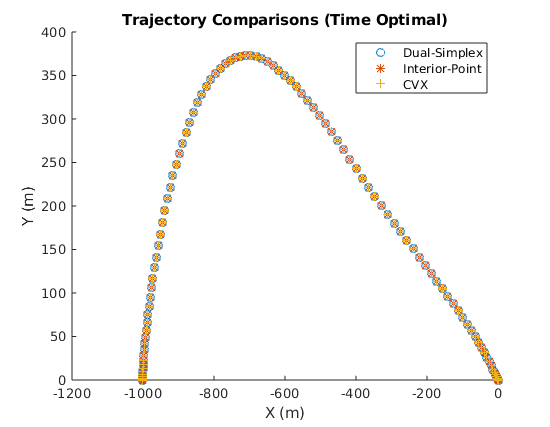
\includegraphics[width=0.7\textwidth]{images/trajectories_time.png}
  \caption{Generated time-optimal trajectories from each solver}
  \label{fig:trajectories-time}
\end{figure}

\begin{figure}[H]
  \centering
  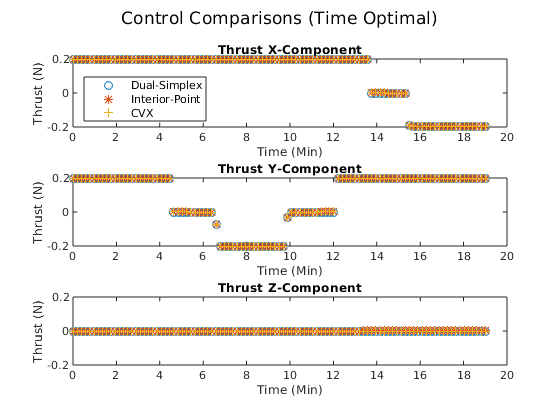
\includegraphics[width=0.7\textwidth]{images/controls_time.png}
  \caption{Generated time-optimal control inputs from each solver}
  \label{fig:controls-time}
\end{figure}

\section*{Conclusion}

The main challenges faced in this project were in formulating the optimization problem - it took several tries before \texttt{Matlab} recognized the L1 slack-variable formulation as an LP.
Additionally,\texttt{ CVX}'s documentation is sparse when it comes to LP problems and it took some time to get a feel for its error messages.
What I learned from this project is both the value of being able to rearrange nonlinear problem components to fit into an LP problem and also that I \textit{vastly} prefer problem-based modeling to calling solver functions like I have in the past.
I spent approximately 8 hours on this project.

\end{document}
